\documentclass{article}

% Listings
\usepackage{listings}
\usepackage{color}
\usepackage{upquote} % preserve backticks

% Fonts
%\usepackage{palatino}
\usepackage{inconsolata}
\usepackage[T1]{fontenc}

% Margin
\usepackage[margin=0.5in]{geometry}

% Images
\usepackage{graphicx}
\graphicspath{ {images/} }


% Colors
\definecolor{comment}{rgb}{0.31,0.31,0.31}
\definecolor{codegray}{rgb}{0.19,0.19,0.19}
\definecolor{string}{rgb}{0.56,0.66,0.35}
\definecolor{backcolor}{rgb}{0.96,0.96,0.96}
\definecolor{keyword}{rgb}{0.67,0.25,0.25}
 
\lstdefinestyle{mystyle}{
    backgroundcolor=\color{backcolor},
    commentstyle=\color{comment},
    keywordstyle=\color{keyword},
    numberstyle=\tiny\color{codegray},
    stringstyle=\color{string},
    basicstyle=\footnotesize\ttfamily,
    breakatwhitespace=false,
    breaklines=true,
    captionpos=t,
    keepspaces=true,
    numbers=left,
    numbersep=5pt,
    showspaces=false,
    showstringspaces=false,
    showtabs=false,
    tabsize=2
}

\lstset{style=mystyle}




\title{Homework 1 - Virtual Machine Scheduling Analysis}
\author{Jared Klingenberger}
\date{February 8, 2016}

\begin{document}

\maketitle

\lstlistoflistings

\section{Rosenblum Paper}

To summarize, Rosenblum's paper on virtual machines is a good overview of the
numerous motivations behind virtual machines. In the early days of virtual
machine computing, a big motivation was for compatibility between different
types of hardware by having a single target abstract machine to code to.
However, a different style of virtual machine made a huge comeback in recent
years with the arrival of VMWare, a hardware-level virtual machine that made it
possible to emulate computer hardware devices. This is quite useful for many
reasons; two such reasons are that these VMs provide superior isolation and that
one can manage the execution of these VMs from a higher level with a Virtual
Machine Manager.

\section{Manual Dataset Creation and Analysis}

Overall for question 2, I noticed that as I increased the blocksize, there
seemed to be noticeable periodic effects in the datasets. So most of the results
would fall around the same value, but some delays were much longer and stacked
around the same times. This likely has something to do with how the scheduler
assigns clock time to different processes. The most noticeable effect can be
seen with blocksize of 1 million.

\subsection{Statistics}

Here are histogram plots and numerical statistics for different blocksizes.

\subsubsection{Blocksize 4}

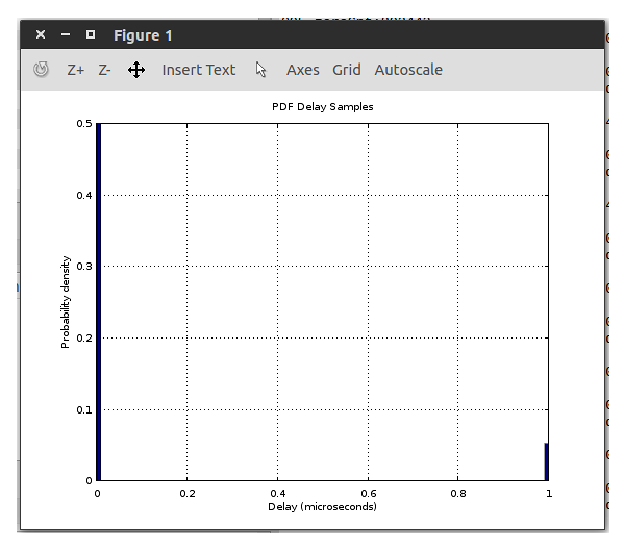
\includegraphics{q2/hw1-4}

\begin{lstlisting}
plotDataPDF (nargin:1):  sampleSize:1000000, maxValue:65.100000,  MAX_ALLOWED_VALUE:1000.000000
#samples:1000000 Mean:     0 microseconds,  median:      0,  std:      0, max:    65, min:     0, maxCount:10173 zeroCnt:947490
percentiles (2.5 25 50 75 97.5): :     0      0      0      0      1
\end{lstlisting}

\subsubsection{Blocksize 256}

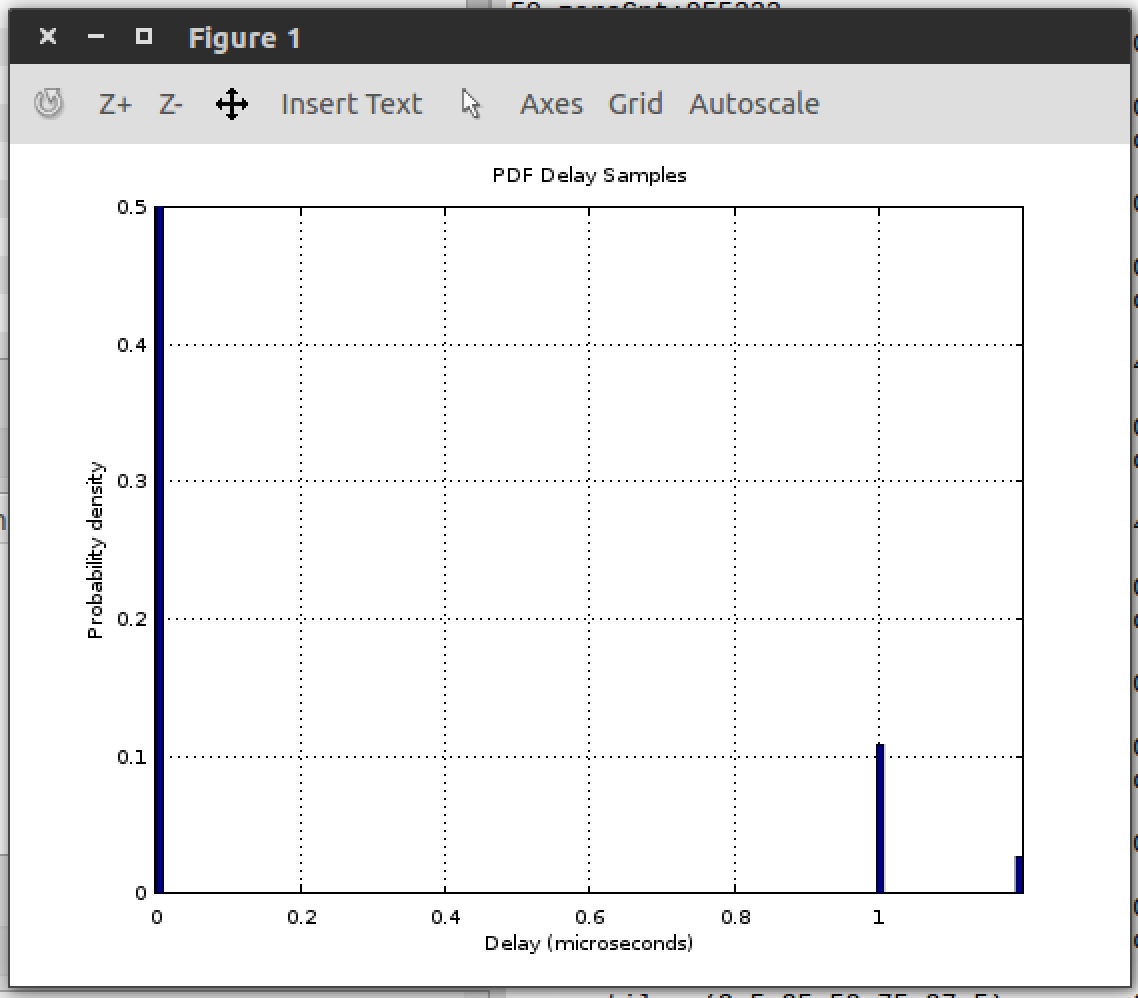
\includegraphics{q2/hw1-256}

\begin{lstlisting}
plotDataPDF (nargin:1):  sampleSize:1000000, maxValue:70.100000,  MAX_ALLOWED_VALUE:1000.000000
#samples:1000000 Mean:     0 microseconds,  median:      0,  std:      0, max:    70, min:     0, maxCount:235 zeroCnt:865266
percentiles (2.5 25 50 75 97.5): :     0      0      0      0      1
\end{lstlisting}

\subsubsection{Blocksize 65535}

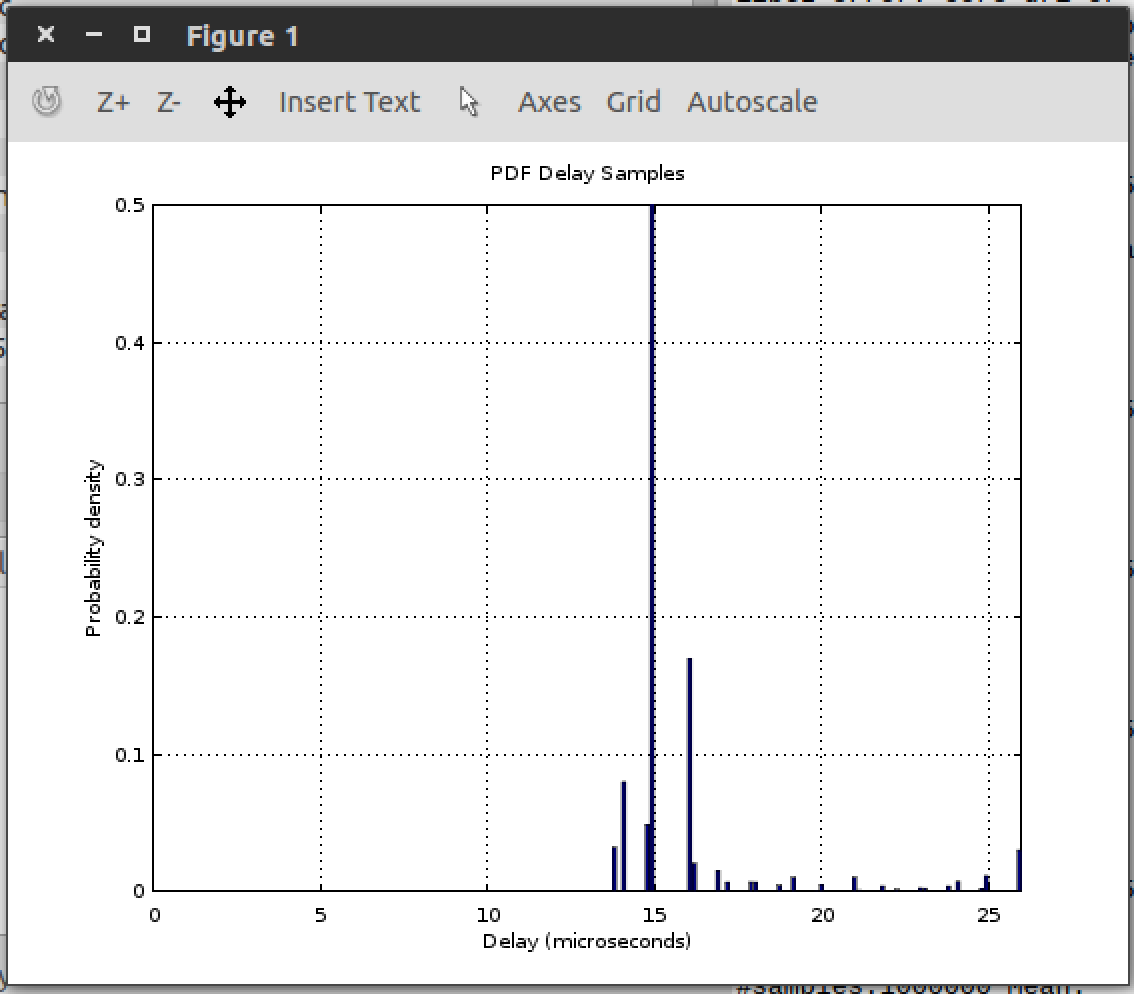
\includegraphics{q2/hw1-65535}

\begin{lstlisting}
plotDataPDF (nargin:1):  sampleSize:1000000, maxValue:4635.100000,  MAX_ALLOWED_VALUE:1000.000000
#samples:1000000 Mean:    16 microseconds,  median:     15,  std:      7, max:  4635, min:    12, maxCount:22358 zeroCnt:0
percentiles (2.5 25 50 75 97.5): :    14     15     15     16     26
\end{lstlisting}

\subsubsection{Blocksize 1000000}

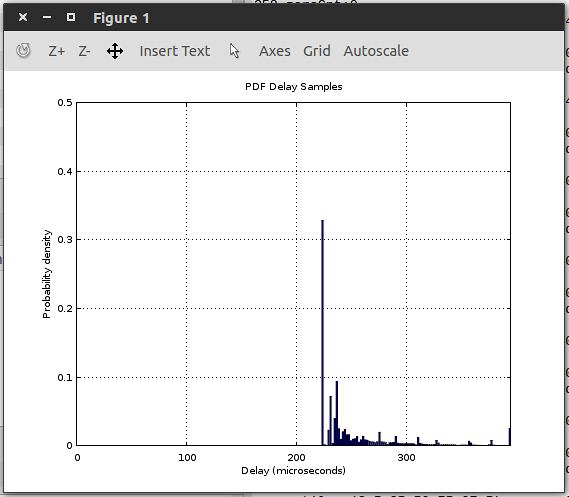
\includegraphics{q2/hw1-1000000}

\begin{lstlisting}
plotDataPDF (nargin:1):  sampleSize:1000000, maxValue:5667.200000,  MAX_ALLOWED_VALUE:1000.000000
#samples:1000000 Mean:   255 microseconds,  median:    236,  std:     51, max:  5667, min:   210, maxCount:24825 zeroCnt:0
percentiles (2.5 25 50 75 97.5): :   223    224    236    263    395
\end{lstlisting}

\subsection{Parallel execution}

I think the programs were completing too quickly to affect mpstat, but I was able to see a spike in CPU usage through using the `top` command.

\begin{lstlisting}
11:30:35 PM  CPU    %usr   %nice    %sys %iowait    %irq   %soft  %steal  %guest  %gnice   %idle
11:30:35 PM  all    0.38    0.00    0.03    0.00    0.00    0.00    0.00    0.00    0.00   99.58
11:30:35 PM    0    0.46    0.00    0.05    0.00    0.00    0.00    0.00    0.00    0.00   99.48
11:30:35 PM    1    0.34    0.01    0.03    0.00    0.00    0.00    0.00    0.00    0.00   99.62
11:30:35 PM    2    0.35    0.00    0.03    0.00    0.00    0.00    0.00    0.00    0.00   99.62
11:30:35 PM    3    0.36    0.00    0.02    0.01    0.00    0.00    0.00    0.00    0.00   99.61
\end{lstlisting}

\subsubsection{Statistics - shell 1}

\begin{lstlisting}
plotDataPDF (nargin:1):  sampleSize:1000000, maxValue:683.100000,  MAX_ALLOWED_VALUE:1000.000000 
#samples:1000000 Mean:     0 microseconds,  median:      0,  std:      1, max:   683, min:     0, maxCount:259 zeroCnt:835032
percentiles (2.5 25 50 75 97.5): :     0      0      0      0      1
\end{lstlisting}

\subsubsection{Statistics - shell 2}

\begin{lstlisting}
plotDataPDF (nargin:1):  sampleSize:1000000, maxValue:90.100000,  MAX_ALLOWED_VALUE:1000.000000 
#samples:1000000 Mean:     0 microseconds,  median:      0,  std:      1, max:    90, min:     0, maxCount:284 zeroCnt:835508
percentiles (2.5 25 50 75 97.5): :     0      0      0      0      1
\end{lstlisting}

\section{Experiments in Parallel VM Scheduling}

\subsection{Experiment 1}

This first experiment was simply an exercise in automating the testing process.
With a blocksize that varies by $2^i, i \in \{1, 2, ..., 20\}$, the runExp.sh
program automatically performs the experiment all at once.

\subsubsection{Overall stats}

\begin{lstlisting}
Experiment 1
1000000 1024 0.400 0.000 2.408
1000000 1048576 287.784 275.900 53.599
1000000 128 0.153 0.000 0.569
1000000 131072 36.570 33.900 17.870
1000000 16 0.082 0.000 1.135
1000000 16384 4.572 4.100 2.826
1000000 2 0.092 0.000 0.493
1000000 2048 0.782 1.000 3.638
1000000 256 0.278 0.000 2.141
1000000 262144 73.582 67.900 18.960
1000000 32 0.061 0.000 0.422
1000000 32768 9.244 8.100 6.677
1000000 4 0.095 0.000 0.630
1000000 4096 1.190 1.000 1.365
1000000 512 0.211 0.000 3.652
1000000 524288 143.082 134.000 32.334
1000000 64 0.084 0.000 1.034
1000000 65536 18.039 16.900 6.872
1000000 8 0.093 0.000 0.495
1000000 8192 2.286 2.100 1.999
\end{lstlisting}

\subsubsection{Statistics - blocksize 1048576}

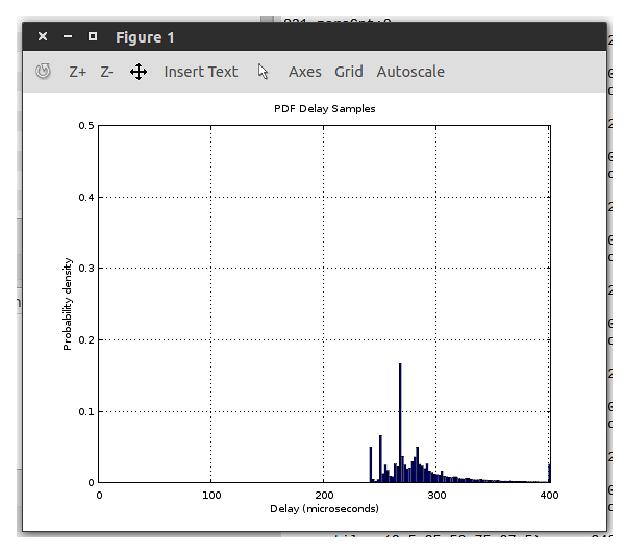
\includegraphics{q3/exp1/bs1m}

\begin{lstlisting}
plotDataPDF (nargin:1):  sampleSize:1000000, maxValue:5829.100000,  MAX_ALLOWED_VALUE:1000.000000
#samples:1000000 Mean:   288 microseconds,  median:    276,  std:     54, max:  5829, min:   184, maxCount:24693 zeroCnt:0
percentiles (2.5 25 50 75 97.5): :   242    267    276    296    402
\end{lstlisting}

\subsubsection{Statistics - blocksize 524288}

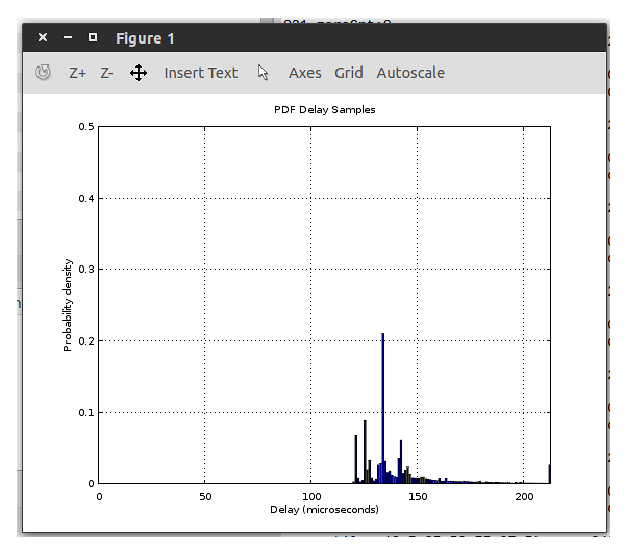
\includegraphics{q3/exp1/bs500k}

\begin{lstlisting}
plotDataPDF (nargin:1):  sampleSize:1000000, maxValue:9854.100000,  MAX_ALLOWED_VALUE:1000.000000
#samples:1000000 Mean:   143 microseconds,  median:    134,  std:     32, max:  9854, min:   107, maxCount:24795 zeroCnt:0
percentiles (2.5 25 50 75 97.5): :   121    132    134    145    213
\end{lstlisting}

\subsubsection{Interpretation}

The results of this experiment are pretty clear. The larger blocksize definitely
has a higher variability, which can be seen visually in the plot by how the
distribution is more spread. This is probably because with more bits to
checksum, there is a higher chance of scheduling affecting the timing with more
granularity.

\subsection{Experiment 2}

Experiment 2 was more interesting because it was meant to do the same thing as
experiment 1, but with the program competing for the CPU by running two
instances of hw1 in parallel. This is what runExp.sh does -- simply runs
experiment 1 twice simultaneously.

\subsubsection{Overall stats - core 1}

\begin{lstlisting}
Experiment 2
1000000 1024 0.396 0.000 7.013
1000000 1048576 287.971 273.900 67.686
1000000 128 0.118 0.000 0.550
1000000 131072 35.803 33.100 14.463
1000000 16 0.078 0.000 1.587
1000000 16384 4.431 4.100 11.559
1000000 2 0.092 0.000 0.430
1000000 2048 0.828 1.000 1.000
1000000 256 0.299 0.000 2.810
1000000 262144 70.562 67.000 19.655
1000000 32 0.049 0.000 0.384
1000000 32768 8.706 8.100 4.817
1000000 4 0.091 0.000 1.428
1000000 4096 1.196 1.000 4.301
1000000 512 0.176 0.000 1.366
1000000 524288 144.228 134.000 36.245
1000000 64 0.080 0.000 1.815
1000000 65536 17.792 16.900 10.709
1000000 8 0.088 0.000 0.429
1000000 8192 2.240 1.900 5.022
\end{lstlisting}

\subsubsection{Overall stats - core 2}
\begin{lstlisting}
Experiment 2
1000000 1024 0.395 0.000 3.535
1000000 1048576 287.680 273.000 65.885
1000000 128 0.118 0.000 0.492
1000000 131072 35.738 33.100 15.173
1000000 16 0.075 0.000 1.518
1000000 16384 4.416 4.100 6.982
1000000 2 0.091 0.000 0.523
1000000 2048 0.831 1.000 3.241
1000000 256 0.284 0.000 2.709
1000000 262144 70.584 67.000 21.541
1000000 32 0.051 0.000 0.405
1000000 32768 8.735 8.100 4.718
1000000 4 0.081 0.000 1.261
1000000 4096 1.203 1.000 7.994
1000000 512 0.174 0.000 0.694
1000000 524288 143.792 134.000 40.463
1000000 64 0.084 0.000 4.540
1000000 65536 17.807 16.900 9.195
1000000 8 0.087 0.000 0.446
1000000 8192 2.237 1.900 5.171
\end{lstlisting}

\subsubsection{Statistics - core 1 (blocksize 1048576)}

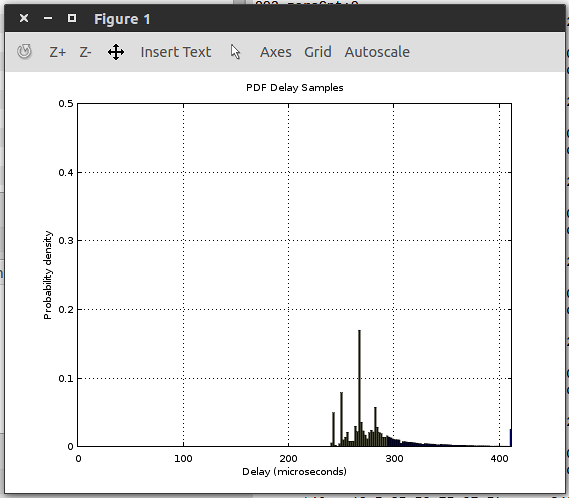
\includegraphics{q3/exp2/core1}

\begin{lstlisting}
plotDataPDF (nargin:1):  sampleSize:1000000, maxValue:22301.900000,  MAX_ALLOWED_VALUE:1000.000000
#samples:1000000 Mean:   288 microseconds,  median:    274,  std:     68, max: 22302, min:   223, maxCount:24821 zeroCnt:0
percentiles (2.5 25 50 75 97.5): :   242    265    274    294    412
\end{lstlisting}

\subsubsection{Statistics - core 2 (blocksize 1048576)}

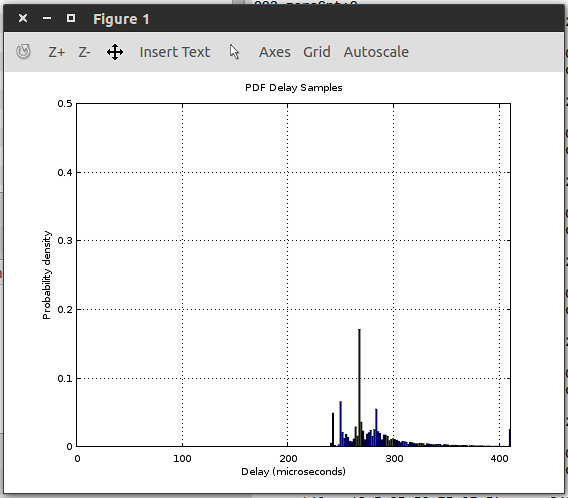
\includegraphics{q3/exp2/core2}

\begin{lstlisting}
plotDataPDF (nargin:1):  sampleSize:1000000, maxValue:25430.000000,  MAX_ALLOWED_VALUE:1000.000000
#samples:1000000 Mean:   288 microseconds,  median:    273,  std:     66, max: 25430, min:   233, maxCount:24657 zeroCnt:0
percentiles (2.5 25 50 75 97.5): :   242    265    273    294    411
\end{lstlisting}

\subsubsection{Interpretation}

In this experiment, the differences were really hard to discern. I didn't notice
any striking changes when scaling up the blocksize, nor when comparing the
statistics of each core. I suspect that this is because my VM had four cores to
work with, thanks to how I configured the VM. In the future, I may want to
increase the number of parallel processes at work.

\subsection{Experiment 3}

This experiment is largly a repeat of experiment 2, but the difference comes in
to how each process is prioritized. I assign one core a nice value of 0 and the
other core a nice value of 19. (Normal users cannot set negative nice values by
default in Ubuntu.)

\subsubsection{Overall stats - core 1}

\begin{lstlisting}
Experiment 3
1000000 1024 0.386 0.000 5.003
1000000 1048576 289.974 272.000 73.226
1000000 128 0.116 0.000 2.633
1000000 131072 37.451 33.900 21.779
1000000 16 0.080 0.000 1.124
1000000 16384 4.463 4.100 4.246
1000000 2 0.096 0.000 0.546
1000000 2048 0.881 1.000 5.817
1000000 256 0.273 0.000 0.611
1000000 262144 72.662 67.000 27.157
1000000 32 0.047 0.000 1.658
1000000 32768 8.811 8.100 6.075
1000000 4 0.092 0.000 2.417
1000000 4096 1.193 1.000 2.703
1000000 512 0.155 0.000 2.092
1000000 524288 141.603 134.000 33.523
1000000 64 0.132 0.000 7.266
1000000 65536 17.985 16.900 12.531
1000000 8 0.090 0.000 1.283
1000000 8192 2.354 1.900 8.776
\end{lstlisting}

\subsubsection{Overall stats - core 2}
\begin{lstlisting}
Experiment 3
1000000 1024 0.385 0.000 3.961
1000000 1048576 290.656 272.000 76.704
1000000 128 0.115 0.000 2.711
1000000 131072 37.443 33.900 27.228
1000000 16 0.060 0.000 1.825
1000000 16384 4.478 4.100 6.304
1000000 2 0.096 0.000 0.549
1000000 2048 0.865 1.000 5.666
1000000 256 0.286 0.000 0.668
1000000 262144 72.529 67.000 29.583
1000000 32 0.042 0.000 1.999
1000000 32768 8.815 8.100 4.721
1000000 4 0.096 0.000 1.277
1000000 4096 1.201 1.000 3.675
1000000 512 0.163 0.000 6.748
1000000 524288 141.794 134.000 40.413
1000000 64 0.071 0.000 1.391
1000000 65536 18.100 16.900 16.403
1000000 8 0.091 0.000 1.125
1000000 8192 2.346 1.900 7.503
\end{lstlisting}

\subsubsection{Statistics - core 1 (blocksize 1048576)}

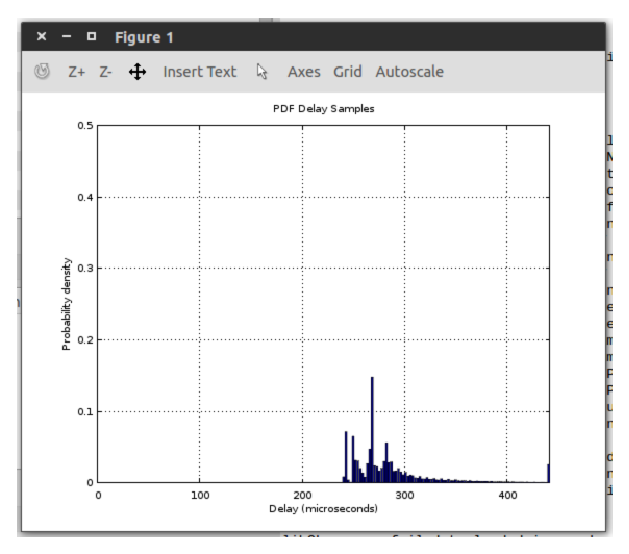
\includegraphics{q3/exp3/core1}

\begin{lstlisting}
plotDataPDF (nargin:1):  sampleSize:1000000, maxValue:7099.900000,  MAX_ALLOWED_VALUE:1000.000000
#samples:1000000 Mean:   290 microseconds,  median:    272,  std:     73, max:  7100, min:   209, maxCount:24881 zeroCnt:0
percentiles (2.5 25 50 75 97.5): :   242    262    272    294    442
\end{lstlisting}

\subsubsection{Statistics - core 2 (blocksize 1048576)}

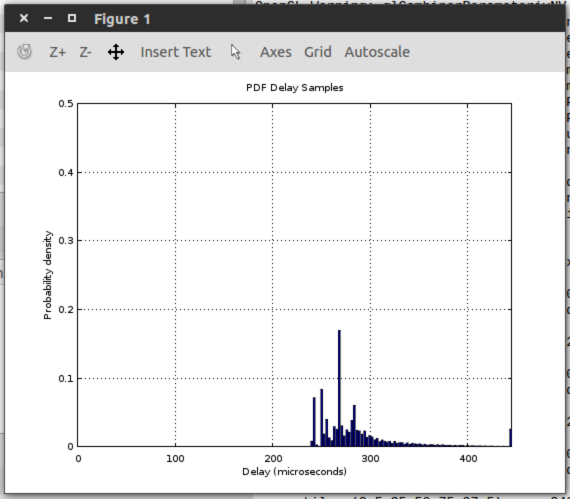
\includegraphics{q3/exp3/core2}

\begin{lstlisting}
plotDataPDF (nargin:1):  sampleSize:1000000, maxValue:12529.900000,  MAX_ALLOWED_VALUE:1000.000000
#samples:1000000 Mean:   291 microseconds,  median:    272,  std:     77, max: 12530, min:   187, maxCount:24902 zeroCnt:0
percentiles (2.5 25 50 75 97.5): :   242    262    272    295    445	
\end{lstlisting}

\subsubsection{Interpretation}

In experiment 3, there was slightly more variability in the lower priority
process. This makes intuitive sense, since the scheduler will have a higher
chance of skipping over the core if other system processes need the processor
more.

\section{Code}

\lstinputlisting[language=c,caption=hw1.c,frame=single,label=code:hw1]{hw1.c}

\lstinputlisting[language=bash,caption=runHW1.sh,frame=single,label=code:runHW1]{runHW1.sh}

\lstinputlisting[language=bash,caption=analysisHW1.sh,frame=single,label=code:analysisHW1]{analysisHW1.sh}

\lstinputlisting[language=awk,caption=analyzeResults.awk,frame=single,label=code:analyzeResults]{analyzeResults.awk}

\end{document}